\documentclass{article}
\usepackage{tikz}
\begin{document}
\begin{center}
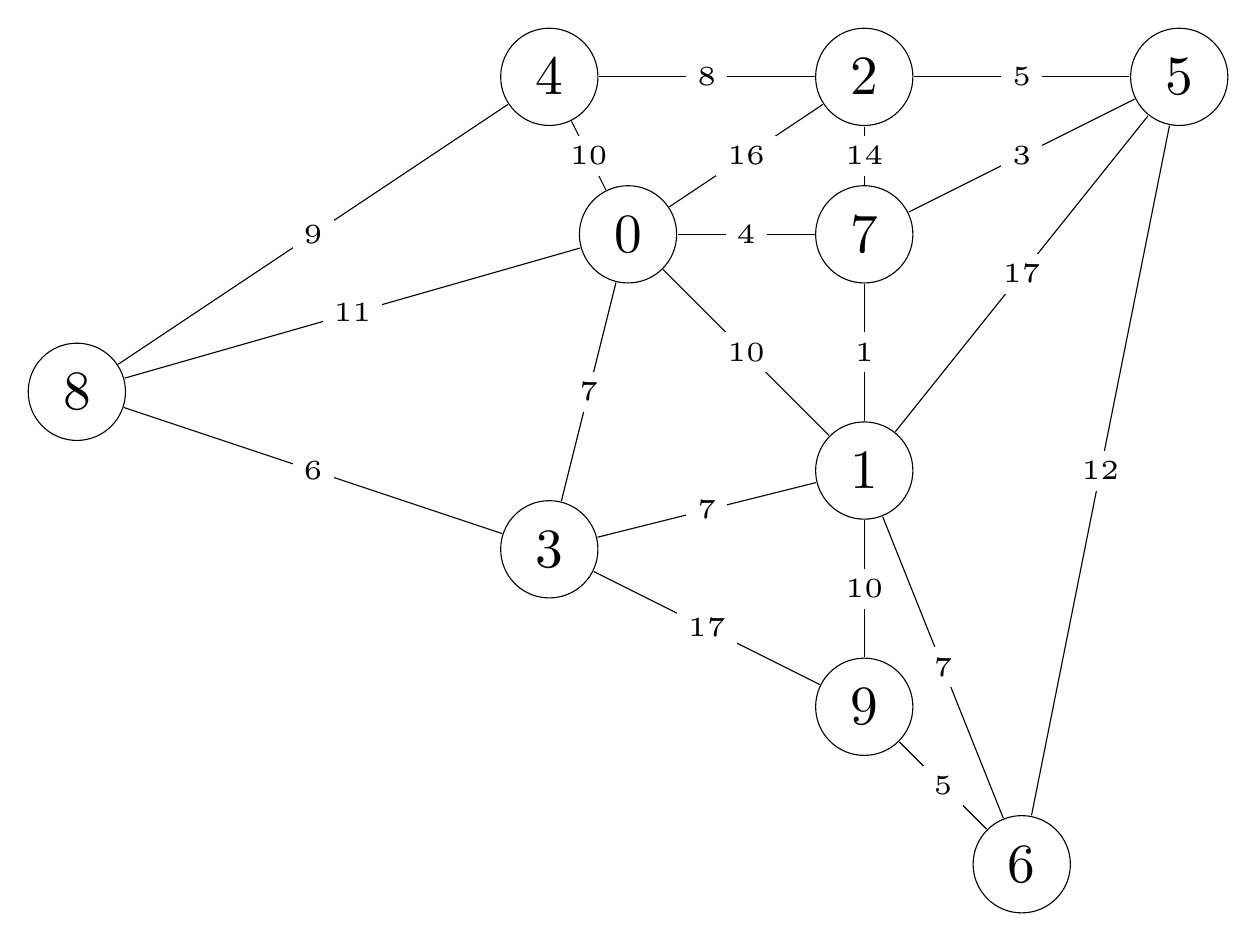
\begin{tikzpicture}[scale=2, transform shape]
% Sommets
\node[draw, circle] (0) at (1.500000, 4.000000) {0};
\node[draw, circle] (1) at (3.000000, 2.500000) {1};
\node[draw, circle] (2) at (3.000000, 5.000000) {2};
\node[draw, circle] (3) at (1.000000, 2.000000) {3};
\node[draw, circle] (4) at (1.000000, 5.000000) {4};
\node[draw, circle] (5) at (5.000000, 5.000000) {5};
\node[draw, circle] (6) at (4.000000, 0.000000) {6};
\node[draw, circle] (7) at (3.000000, 4.000000) {7};
\node[draw, circle] (8) at (-2.000000, 3.000000) {8};
\node[draw, circle] (9) at (3.000000, 1.000000) {9};
\draw (5) -- (6);
\node[fill=white, inner sep=2pt, text=black, font=\tiny] at (4.50, 2.50) {12};
\draw (0) -- (1);
\node[fill=white, inner sep=2pt, text=black, font=\tiny] at (2.25, 3.25) {10};
\draw (8) -- (3);
\node[fill=white, inner sep=2pt, text=black, font=\tiny] at (-0.50, 2.50) {6};
\draw (3) -- (9);
\node[fill=white, inner sep=2pt, text=black, font=\tiny] at (2.00, 1.50) {17};
\draw (2) -- (7);
\node[fill=white, inner sep=2pt, text=black, font=\tiny] at (3.00, 4.50) {14};
\draw (0) -- (4);
\node[fill=white, inner sep=2pt, text=black, font=\tiny] at (1.25, 4.50) {10};
\draw (7) -- (1);
\node[fill=white, inner sep=2pt, text=black, font=\tiny] at (3.00, 3.25) {1};
\draw (4) -- (8);
\node[fill=white, inner sep=2pt, text=black, font=\tiny] at (-0.50, 4.00) {9};
\draw (1) -- (5);
\node[fill=white, inner sep=2pt, text=black, font=\tiny] at (4.00, 3.75) {17};
\draw (1) -- (3);
\node[fill=white, inner sep=2pt, text=black, font=\tiny] at (2.00, 2.25) {7};
\draw (6) -- (9);
\node[fill=white, inner sep=2pt, text=black, font=\tiny] at (3.50, 0.50) {5};
\draw (4) -- (2);
\node[fill=white, inner sep=2pt, text=black, font=\tiny] at (2.00, 5.00) {8};
\draw (7) -- (0);
\node[fill=white, inner sep=2pt, text=black, font=\tiny] at (2.25, 4.00) {4};
\draw (1) -- (6);
\node[fill=white, inner sep=2pt, text=black, font=\tiny] at (3.50, 1.25) {7};
\draw (8) -- (0);
\node[fill=white, inner sep=2pt, text=black, font=\tiny] at (-0.25, 3.50) {11};
\draw (2) -- (5);
\node[fill=white, inner sep=2pt, text=black, font=\tiny] at (4.00, 5.00) {5};
\draw (0) -- (2);
\node[fill=white, inner sep=2pt, text=black, font=\tiny] at (2.25, 4.50) {16};
\draw (9) -- (1);
\node[fill=white, inner sep=2pt, text=black, font=\tiny] at (3.00, 1.75) {10};
\draw (7) -- (5);
\node[fill=white, inner sep=2pt, text=black, font=\tiny] at (4.00, 4.50) {3};
\draw (0) -- (3);
\node[fill=white, inner sep=2pt, text=black, font=\tiny] at (1.25, 3.00) {7};
\end{tikzpicture}
\end{center}
\end{document}
